% ctex加载了[no-math]{fontspec},字体不对数学公式生效
% 而mathspec也加载了fontspec所以会报错需要在\documentclass之前采取以下命令
\PassOptionsToPackage{no-math}{fontspec}

\documentclass[UTF8,twoside,zihao=-4]{ctexbook}

% Set page size and margins
\usepackage[a4paper,margin=3cm]{geometry}

% Useful packages
\usepackage{amsmath}
\usepackage{graphicx}

%------------------------------------超链接-------------------------------------------%
\usepackage[colorlinks,linkcolor=black,anchorcolor=black,citecolor=black,filecolor=black,urlcolor=black,runcolor=black,menucolor=black,CJKbookmarks=True]{hyperref}

%---------------------------------设置字号,参见xeCJK----------------------------------%
%\baselineskip=1.56倍
\usepackage{lmodern} % 字号修正
%\newcommand{\chuhao}{\fontsize{42bp}{\baselineskip}\selectfont}     %初号
\newcommand{\xiaochuhao}{\fontsize{36bp}{36pt}\selectfont}           %小初号
%\newcommand{\yihao}{\fontsize{26bp}{\baselineskip}\selectfont}      %一号
\newcommand{\erhao}{\fontsize{22bp}{\baselineskip}\selectfont}       %二号 
\newcommand{\xiaoerhao}{\fontsize{18bp}{\baselineskip}\selectfont}   %小二号
\newcommand{\sanhao}{\fontsize{16bp}{1.2\baselineskip}\selectfont}      %三号
\newcommand{\xiaosanhao}{\fontsize{15bp}{\baselineskip}\selectfont}  %小三号
%\newcommand{\sihao}{\fontsize{14bp}{\baselineskip}\selectfont}		 %四号
\newcommand{\xiaosihao}{\fontsize{12bp}{\baselineskip}\selectfont}   %小四号
\newcommand{\wuhao}{\fontsize{10.5bp}{\baselineskip}\selectfont}    %五号
\newcommand{\xiaowuhao}{\fontsize{9bp}{\baselineskip}\selectfont}    %小五号
%\newcommand{\liuhao}{\fontsize{7.5bp}{\baselineskip}\selectfont}    %六号
%\newcommand{\qihao}{\fontsize{5.5bp}{\baselineskip}\selectfont}     %七号

%--------------------------------设置全局字体,参见xeCJK-------------------------------%
\usepackage{mathspec}
% 英文字体
\setmainfont[AutoFakeBold,AutoFakeSlant]{Times New Roman} % Times New Roman
%\setsansfont{DejaVu Sans}
%\setmonofont{Latin Modern Mono}

% 中文字体
\setCJKmainfont[Path=./fonts/,AutoFakeBold,AutoFakeSlant]{songti.ttc} % 宋体
%\setCJKsansfont{SimHei}
%\setCJKmonofont{SimSun}
%\punctstyle{kaiming}     % 不使用标点独占一格的行为

% 数学字体
\xeCJKDeclareCharClass{CJK}{`0 -> `9} % 设置 0-9 以 CJK 字体输出;用中文字体显示阿拉伯数字,这样数字就总是和周围的汉字使用相同的字体
%\normalspacedchars{0,1,2,3,4,5,6,7,8,9} % 还原0-9 的字符类

%-----------------------------设置其他字体,参见xeCJK----------------------------------%
\newCJKfontfamily[hwzs]\hwzs{huawenzhongsong.TTF}[Path=./fonts/,AutoFakeBold,AutoFakeSlant]  % 华文中宋 假黑体
\newCJKfontfamily[hwfs]\hwfs{huawenfangsong.TTF}[Path=./fonts/,AutoFakeBold,AutoFakeSlant]   % 华文仿宋 假黑体
\newCJKfontfamily[fsgb]\fsgb{fangsonggb2312.ttf}[Path=./fonts/,AutoFakeBold,AutoFakeSlant]   % 仿宋GB2312 假黑体
\newCJKfontfamily[heit]\heit{heiti.ttf}[Path=./fonts/,AutoFakeBold,AutoFakeSlant]			 % 黑体 假黑体

%----------------------------------设置图表标题格式-------------------------------------%
\usepackage{caption}
\DeclareCaptionFont{heit}{\heit} % 声明字体
\DeclareCaptionFont{wuhao}{\wuhao} % 声明字号

\renewcommand{\thetable}{\thechapter-\arabic{table}} % 设置标签编号的格式
\renewcommand{\thefigure}{\thechapter-\arabic{figure}}
\captionsetup{
%	format = plain,% 设置长标题格式
	labelformat = simple, % 设置标签编号的格式
	labelsep = quad, % 标签与后面标题之间的间隔
	justification = centering, % 设置浮动标题的对齐方式
	font={heit,wuhao,bf,singlespacing}, % 设置浮动标题的字体
	skip=0.5\baselineskip, % 控制标题与浮动环境内容的垂直间距
	figurename=图, % 设置标题标签的文字名称
	tablename=表,
}


%------------------------------页眉页脚,参见fancyhdr----------------------------------%
\usepackage{fancyhdr}
\usepackage{emptypage}
\fancypagestyle{qianyan}{
	\fancyhf{} % 清除页眉页脚
	\pagenumbering{arabic} % 页码格式
	\fancyfoot[C]{\xiaowuhao \bfseries \thepage}
	\renewcommand{\headrulewidth}{0pt}
	\renewcommand{\footrulewidth}{0pt}
}
\fancypagestyle{plain}{
	\fancyhf{} % 清除页眉页脚
	\fancyfoot[C]{\xiaowuhao \bfseries \thepage}
	\renewcommand{\headrulewidth}{0pt}
	\renewcommand{\footrulewidth}{0pt}
}

%----------------------    自定义封面(包括学术声明)    --------------------------------%
\renewcommand{\maketitle}{
	\pagestyle{empty} % 清除该部分页码\pagestyle是该页及以后
	\begin{titlepage}
%-------------------------------------      封面    -----------------------------------%
% logo
		{
			\noindent % 临时取消首行缩进
			
\includegraphics[width=0.7\linewidth]{pic_of_cover/swufelogo.png}
		}

		\vspace{64pt} % 留空白

		\begin{center}
% 首页带有届数的黑标题
			{
				\xiaochuhao % 小初号字
				\heit % 黑体
				\bfseries % 加粗黑体
				2023~届\\
				本科毕业论文(设计)\\
			}
			
			\vspace{66.5pt} % 留空白
% 题目作者等信息
			{
				\sanhao % 三号字 1.5倍行距
				\def\coveritem##1:##2 {
					{\fsgb \bfseries ##1}&{\hwfs \CJKunderline[thickness=1pt] {\centerline{##2}}} \\}
				\begin{tabular}{lp{0.8\linewidth}}
					\coveritem {论文题目:}:{新形势下企业金融风险管理探析} % 支持22字符,过多需要启用下一行
%					\coveritem :{新形势下企业金融风险管理探析MMMMMMMM}
					\coveritem {学生姓名:}:{陈朵朵}
					\coveritem {所在学院:}:{学不会学院}
					\coveritem {专\hspace{2em}业:}:{不会学}
					\coveritem {学\hspace{2em}号:}:{41928999}
					\coveritem {指导教师:}:{张指导}
					\coveritem {成\hspace{2em}绩:}:{}
				\end{tabular}
			}

			\vspace{\fill}
% 封面的日期
			{
				\sanhao % 三号字
				\hwfs % 华文仿宋
				\bfseries % 加粗华文仿宋
				\number\year~年~\number\month~月 % 当前日期
			}
		\end{center}

%--------------------------------         学术声明       ---------------------%
	\cleardoublepage % 新的一页
	\vspace*{\baselineskip} % 大字前留空白
% 大标题
	\begin{center}
		\bfseries \hwzs \xiaoerhao% 粗体 华文中宋 小二号字
		西南财经大学\\
		本科毕业论文原创性及知识产权声明
	\end{center}

	\vspace{15.6pt}

% 声明正文
	\xiaosihao
	本人郑重声明:所呈交的毕业论文是本人在导师的指导下取得的成果,论文
	写作严格遵循学术规范。对本论文的研究做出重要贡献的个人和集体,均已在文
	中以明确方式标明。因本毕业论文引起的法律结果完全由本人承担。
	
	本毕业论文成果归西南财经大学所有。
	
	\vspace{15.6pt} % 空行
	
	特此声明

	\vspace{156pt}
	
% 签字处
	\begin{flushright}
		毕业论文作者签名:\hspace*{5em} \\
		作者专业:\hspace*{5em} \\
		作者学号:\hspace*{5em} \\
		\number\year~年~\number\month~月~\number\day~日
	\end{flushright}
	\end{titlepage}
}


%--------------------------------       中文摘要            --------------------------%
\newenvironment{abstract}[1]{%
	\cleardoublepage
	\thispagestyle{qianyan} % 页码\thispagestyle是当前页
	\newcommand{\keywords}{#1} % 关键词的传递
% 摘要俩大字
	{
		\vspace*{\baselineskip}
		\erhao \hwzs \bfseries \centerline{摘要}
		\vspace{\baselineskip}
		\addcontentsline{toc}{part}{摘要} % 不想在目录中出现摘要可将改行注释掉
	}
% 摘要正文的字体
	\xiaosihao \bfseries
}{
	\vspace{\baselineskip}
	
	{
		\noindent % 取消缩进
		\textbf{关键词:{\keywords}}
	}
}

%---------------------------------        英文摘要       -----------------------------%
\newenvironment{abstracten}[1]{%
	\cleardoublepage
	\thispagestyle{qianyan} % 页码
	\newcommand{\keywords}{#1} % 关键词的传递
	{
		\vspace*{\baselineskip}
		\erhao \bfseries \centerline{Abstract}
		\vspace{\baselineskip}
		\addcontentsline{toc}{part}{Abstract} % 不想在目录中出现摘要可将改行注释掉
	}
	\xiaosihao \bfseries
}{
	\vspace{\baselineskip}
	
	{
		\noindent % 取消缩进
		\textbf{Keywords:{\keywords}}
	}
}

%--------------     目录格式,参见The Short Introduction to LaTeX2e     ---------------%
\renewcommand{\contentsname}{
	\vspace*{-3\baselineskip} % 因为目录是一个\chapter造成空白太大,所以要升高位置
	\erhao \hwzs \bfseries % 二号 华文中宋 加粗
	目录
}
\usepackage{titletoc}
\titlecontents{part} % 用来设置参考文献等的目录格式
[0em] % 左间距
{\fontsize{12bp}{1.3\baselineskip}\selectfont \bfseries} % 标题格式
{} % 序号格式
{} % 没有序号的标题
{\titlerule*[0.7pc]{$\cdot$}\contentspage\hfill} % 指引线与页码

\titlecontents{chapter}
[2em]
{\xiaosihao \bfseries}
{\contentslabel{2em}}
{}
{\titlerule*[0.7pc]{$\cdot$}\contentspage\hfill}

\titlecontents{section}
[4em] % 左间距
{\xiaosihao} % 标题格式
{\contentslabel{2em}} % 序号格式
{} % 没有序号的标题
{\titlerule*[0.7pc]{$\cdot$}\contentspage\hfill} % 指引线与页码

\titlecontents{subsection}
[7em] % 左间距
{\xiaosihao} % 标题格式
{\contentslabel{3em}} % 序号格式
{} % 没有序号的标题
{\titlerule*[0.7pc]{$\cdot$}\contentspage\hfill} % 指引线与页码

%======================全角半角标点========================
% punct = ⟨quanjiao|banjiao|kaiming|CCT|plain⟩
%========是否保留汉字后的空格===================
% space = ⟨true|false|auto⟩
%=======================字号变化时是否自动调整首段缩进===============
% autoindent = ⟨true|false|数值|带单位的数值⟩

%======================对齐===============================
% linestretch = ⟨数值或长度⟩


%--------------------------------    正文标题,参见CTEX     ---------------------------%
\ctexset{
	chapter={ % 一级标题
		number = \arabic{chapter},
		name = {,.},
		format = \erhao \hwzs \bfseries \centering,
		beforeskip = {3\baselineskip}, 
		afterskip = {2\baselineskip}, 
	},
	section={ % 二级标题
		name = {},
		format =  \xiaosanhao \heit,
		beforeskip = {1\baselineskip}, 
		afterskip = {1\baselineskip}, 
	},
	subsection={ % 三级标题
		name = {},
		format = \heit,
		beforeskip = {1\baselineskip}, 
		afterskip = {1\baselineskip},
	},
}

%------------------------------------   参考文献    -----------------------------------%
\usepackage[style=gb7714-2015,sorting=gb7714-2015,doi=false,isbn=false,url=false,eprint=false,gbpub=false,]{biblatex}
% 引入参考文献的数据
\addbibresource{refs.bib}


%---------------------------------   附录和致谢   -------------------------------------%
\newenvironment{fulu}[1][附录]{
	\chapter*{#1}
	\addcontentsline{toc}{part}{#1} % 不想在目录中出现可将此行注释掉
}{}

\newenvironment{acknowledgments}[1][致谢]{
	\chapter*{#1}
	\addcontentsline{toc}{part}{#1} % 不想在目录中出现可将此行注释掉
}{}

%------------------------------------   封底   ---------------------------------------%
\usepackage{tikz}
\newcommand{\backcover}{
	\cleardoublepage
	\pagestyle{empty} % 清除该部分页码\pagestyle是该页及以后
	\noindent % 临时取消首行缩进
	\hfill
	\newpage
	%放页面中心,原始图片
	\begin{tikzpicture}[overlay,remember picture]
		\node(1)[xshift=0cm,yshift=0cm] at (current page.center) {
			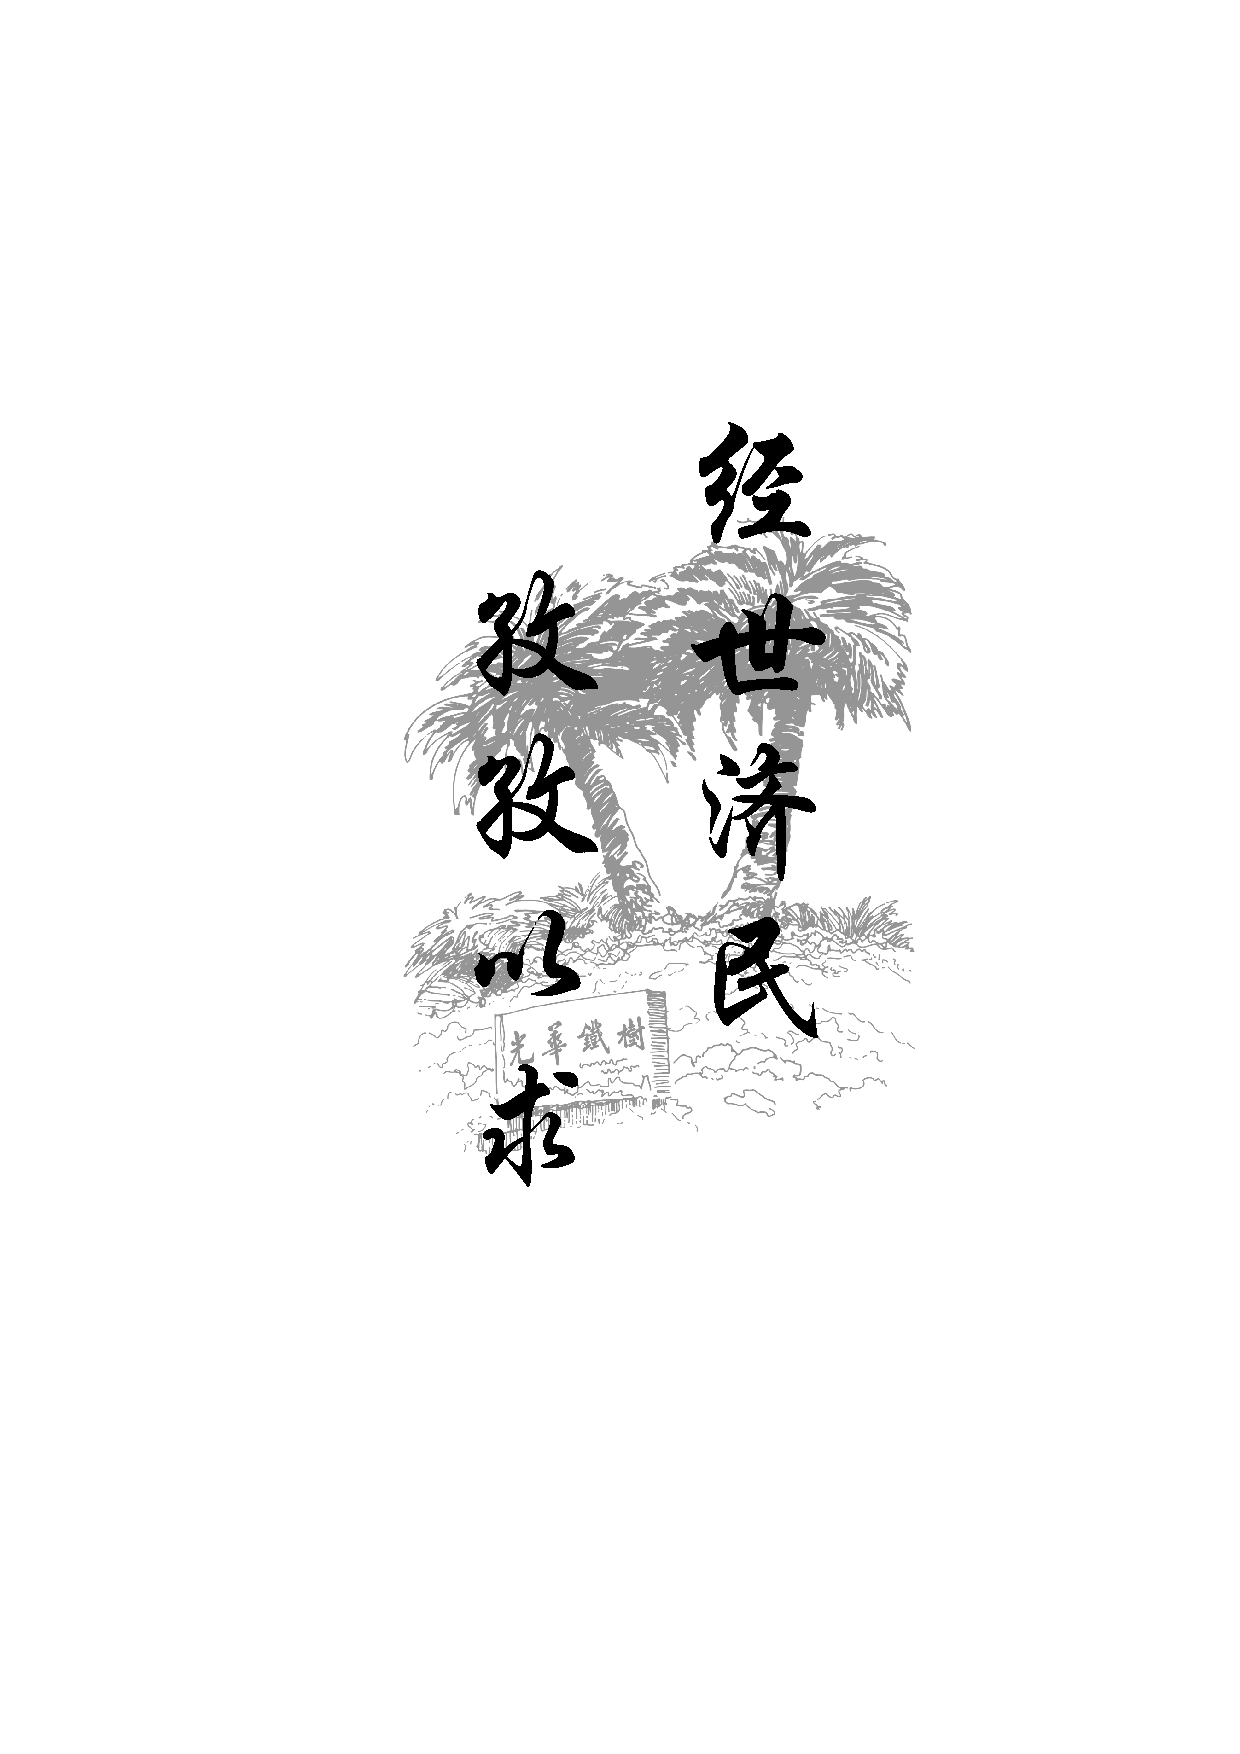
\includegraphics[width=8.66cm]{pic_of_cover/backcover.pdf}};
	\end{tikzpicture}
	}

%--------------------------------   正文   ----------------------------------------%
\begin{document}
	\maketitle % 打印封面和学术声明

%-----------------------------------  中英摘要  -------------------------------------
	
	\begin{abstract}{
			关键词;哈哈哈;分号隔开;最后没有分号
		} % 中文摘要
	
		摘要摘要
		$ a_1^s=123^2a $wedwesxc111
		
		关键词巴拉巴拉巴拉巴拉巴拉en
	\end{abstract}
	
	\begin{abstracten}{
			fenhao;Keywords;las  tisnot
		} % 英文摘要
		摘要摘要
		$ a_1^s=123^2a $wedwesxc111
		
		关键词巴拉巴拉巴 拉巴拉巴拉en
	\end{abstracten}

%------------------------------------   目录  ------------------------------------

	\frontmatter %前言部分,页码为小写罗马字母格式;其后的\chapter 不编号。
	\tableofcontents %目录
	\thispagestyle{qianyan}
	
%--------------------------------------  正文 --------------------------------------
	\mainmatter    %表示开始正文部分的内容 使用数字进行页面编号,对其中的chapter进行编号
	\pagestyle{plain} % 设置与\part\chapter所在页面的格式相同
	
	\chapter{二号华文中宋加粗}
	
	\section{小三号黑体}
	哈哈哈哈哈哈哈哈哈哈哈哈,哈哈哈哈哈哈哈哈哈哈哈哈哈哈哈?哈哈哈哈哈哈哈哈哈哈哈哈哈哈哈哈哈哈哈哈哈哈,哈,哈,哈哈,哈,哈,哈,哈:,哈“,哈哈哈哈哈哈哈哈哈哈哈哈哈哈哈哈哈哈哈哈哈哈哈哈哈哈哈哈哈哈哈哈哈哈哈哈哈哈哈哈哈哈哈哈哈哈哈哈哈哈哈哈哈\%哈吼吼吼吼吼吼吼吼吼吼吼吼吼吼吼
	哈哈哈哈\cite{2009}
	
	哈哈哈哈哈哈哈哈哈哈哈哈哈哈哈哈哈哈哈
	\section{无线通信信道研究概况}
	哈哈哈哈哈哈哈哈哈哈哈哈哈哈哈哈哈哈哈哈哈哈哈哈哈哈哈哈哈哈哈哈哈哈哈哈哈哈哈哈哈哈哈哈哈哈哈哈哈哈哈哈哈哈哈哈哈哈哈哈哈哈哈哈哈哈哈哈哈哈哈哈哈哈哈哈哈哈哈哈哈哈哈哈哈哈哈哈哈哈哈哈哈哈哈哈哈哈哈哈哈哈哈哈哈哈哈哈哈哈哈哈吼吼吼吼吼吼吼吼吼吼吼吼吼吼吼
	哈哈哈哈
	\section{无线通信信道模型的介绍}
	哈哈哈哈哈哈哈哈哈哈哈哈哈哈哈哈哈哈哈哈哈哈哈哈哈哈哈哈哈哈哈哈哈哈哈哈哈哈哈哈哈哈哈哈哈哈哈哈哈哈哈哈哈哈哈哈哈哈哈哈哈哈哈哈哈哈哈哈哈哈哈哈哈哈哈哈哈哈哈哈哈哈哈哈哈哈哈哈哈哈哈哈哈哈哈哈哈哈哈哈哈哈哈哈哈哈哈哈哈哈哈哈吼吼吼吼吼吼吼吼吼吼吼吼吼吼吼
	哈哈哈哈
	\section{论文设计任务}
	哈哈哈哈哈哈哈哈哈哈哈哈哈哈哈哈哈哈哈哈哈哈哈哈哈哈哈哈哈哈哈哈哈哈哈哈哈哈哈哈哈哈哈哈哈哈哈哈哈哈哈哈哈哈哈哈哈哈哈哈哈哈哈哈哈哈哈哈哈哈哈哈哈哈哈哈哈哈哈哈哈哈哈哈哈哈哈哈哈哈哈哈哈哈哈哈哈哈哈哈哈哈哈哈哈哈哈哈哈哈哈哈吼吼吼吼吼吼吼吼吼吼吼吼吼吼吼
	哈哈哈哈
	\section{本文结构安排}
	哈哈哈哈哈哈哈哈哈哈哈哈哈哈哈哈哈哈哈哈哈哈哈哈哈哈哈哈哈哈哈哈哈哈哈哈哈哈哈哈哈哈哈哈哈哈哈哈哈哈哈哈哈哈哈哈哈哈哈哈哈哈哈哈哈哈哈哈哈哈哈哈哈哈哈哈哈哈哈哈哈哈哈哈哈哈哈哈哈哈哈哈哈哈哈哈哈哈哈哈哈哈哈哈哈哈哈哈哈哈哈哈吼吼吼吼吼吼吼吼吼吼吼吼吼吼吼
	哈哈哈哈\footnote{了了了了了了了了}
	
	\chapter{第二章}
	
	\section{Introduction}
	
\begin{figure}
	\centering
	
\includegraphics[width=0.7\linewidth]{pic_of_cover/swufelogo}
	\caption{fig:swufelogo}
	\label{fig:swufelogo}
\end{figure}
	
\begin{figure}
	\centering
	
\includegraphics[width=0.7\linewidth]{pic_of_cover/swufelogo}
	\caption{哈哈哈哈哈felogo}
	\label{fig:swufelogo}
\end{figure}
	
	\section{无线通信信道模型的介绍}
	哈哈哈哈哈哈哈哈哈哈哈哈哈哈哈哈哈哈哈哈哈哈哈哈哈哈哈哈哈哈哈哈哈哈哈哈哈哈哈哈哈哈哈哈哈哈哈哈哈哈哈哈哈哈哈哈哈哈哈哈哈哈哈哈哈哈哈哈哈哈哈哈哈哈哈哈哈哈哈哈哈哈哈哈哈哈哈哈哈哈哈哈哈哈哈哈哈哈哈哈哈哈哈哈哈哈哈哈哈哈哈哈吼吼吼吼吼吼吼吼吼吼吼吼吼吼吼
	
	$ \dfrac{1}{PF_R^2}=\sigma $\fullcite{2002}
	
	哈哈哈哈
	\section{论文设计任务}
	哈哈哈哈哈哈哈哈哈哈哈哈哈哈哈哈哈哈哈哈哈哈哈哈哈哈哈哈哈哈哈哈哈哈哈哈哈哈哈哈哈哈哈哈哈哈哈哈哈哈哈哈哈哈哈哈哈哈哈哈哈哈哈哈哈哈哈哈哈哈哈哈哈哈哈哈哈哈哈哈哈哈哈哈哈哈哈哈哈哈哈哈哈哈哈哈哈哈哈哈哈哈哈哈哈哈哈哈哈哈哈哈吼吼吼吼吼吼吼吼吼吼吼吼吼吼吼
	哈哈哈哈
	\subsection{本文结构安排}
	哈哈哈哈哈哈哈哈哈哈哈哈哈哈哈哈哈哈哈哈哈哈哈哈哈哈哈哈哈哈哈哈哈哈哈哈哈哈哈哈哈哈哈哈哈哈哈哈哈哈哈哈哈哈哈哈哈哈哈哈哈哈哈哈哈哈哈哈哈哈哈哈哈哈哈哈哈哈哈哈哈哈哈哈哈哈哈哈哈哈哈哈哈哈哈哈哈哈哈哈哈哈哈哈哈哈哈哈哈哈哈哈吼吼吼吼吼吼吼吼吼吼吼吼吼吼吼
	哈哈哈哈

	哈哈哈哈哈哈哈哈哈哈哈哈哈哈哈哈哈哈哈哈哈哈哈哈哈哈哈哈哈哈哈哈哈哈哈哈哈哈哈哈哈哈哈哈哈哈哈哈哈哈哈哈哈哈哈哈哈哈哈哈哈哈哈哈哈哈哈哈哈哈哈哈哈哈哈哈哈哈哈哈哈哈哈哈哈哈哈哈哈哈哈哈哈哈哈哈哈哈哈哈哈哈哈哈哈哈哈哈哈哈哈哈吼吼吼吼吼吼吼吼吼吼吼吼吼吼吼
	
	QQQQQ\cite{2009}哈哈哈哈哈哈哈哈哈哈吼吼
	
	哈哈哈哈
	\section{本文结构安排}
	哈哈哈哈哈哈哈哈哈哈哈哈哈哈哈哈哈哈哈哈哈哈哈哈哈哈哈哈哈哈哈哈哈哈哈哈哈哈哈哈哈哈哈哈哈哈哈哈哈哈哈哈哈哈哈哈哈哈哈哈哈哈哈哈哈哈哈哈哈哈哈哈哈哈哈哈哈哈哈哈哈哈哈哈哈哈哈哈哈哈哈哈哈哈哈哈哈哈哈哈哈哈哈哈哈哈哈哈哈哈哈哈吼吼吼吼吼吼吼吼吼吼吼吼吼吼吼
	哈哈哈哈
		% Table generated by Excel2LaTeX from sheet 'Sheet1'
	\begin{table}[htbp]
		\centering
		\caption{Add caption}
		\begin{tabular}{lr}
			
			q     & 1 \\
			w     & 1 \\
			e     & 2 \\
			r     & 6 \\
			t     & 3 \\
			
		\end{tabular}%
		\label{tab:addlabel}%
	\end{table}%
	
	\chapter{第3章}
	
		% Table generated by Excel2LaTeX from sheet 'Sheet1'
	\begin{table}[htbp]
		\centering
		\caption{Add caption}
		\begin{tabular}{lr}
			
			q     & 1 \\
			w     & 1 \\
			e     & 2 \\
			r     & 6 \\
			t     & 3 \\
			
		\end{tabular}%
		\label{tab:addlabel}%
	\end{table}%
	
	{\heit 哈哈 \textit{哈哈} \textbf{哈}}
	
%--------------------------------------总结和附录--------------------------------------
	\backmatter %后记部分,页码格式不变,继续正常计数;其后的\chapter 不编号。
	
	
% BibLaTeX打印参考文献
	\printbibliography
	\addcontentsline{toc}{part}{参考文献} % 不想在目录中出现摘要可将改行注释掉

% 附录
	\appendix
	\begin{fulu}
		附录
		
		表格
		
		谢辞应以简短的文字对课题研究与论文撰写过程中曾直接给予帮助的人员(例如指导教师、答疑教师及其他人员)表示对自己的谢意,这不仅是一种礼貌,也是对他人劳动的尊重,是治学者应当遵循的学术规范。内容限一页。
	\end{fulu}
		
% 致谢
\begin{acknowledgments}
	谢辞应以简短的文字对课题研究与论文撰写过程中曾直接给予帮助的人员(例如指导教师、答疑教师及其他人员)表示对自己的谢意,这不仅是一种礼貌,也是对他人劳动的尊重,是治学者应当遵循的学术规范。内容限一页。
\end{acknowledgments}

\backcover

\end{document}